\lecture{Sept. 29}

\begin{defn}
We sat that $\{a_n\}$ diverges to $\infty$ if for every $M\geq 0$ there exists $N_0\in \mathbb{N}$ such that if $n\geq N_0$, then $a_n>M$

We write $$\lim_{n\to \infty} a_n = \infty$$
\end{defn}


\begin{figure}[ht]
\centering
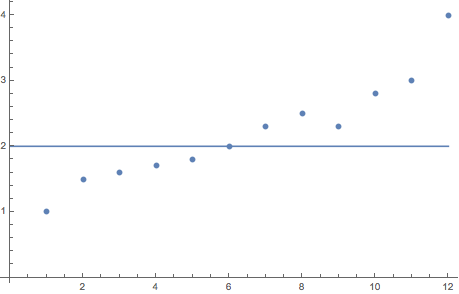
\includegraphics[width=0.6\textwidth]{picture/2.png}
\caption{$\{a_n\}$ and $M=2$}
\end{figure}

\begin{ques}
Does every sequence $\{a_n\}$ that is \underline{not} bounded above diverges to $\infty$? 
\end{ques} 

No. $\{0,1,0,2,0,3,0,4,0,5,\dots\}$

\begin{note}
 If $\{a_n\}$ is non-decreasing then either 
\begin{enumerate}
\item[1)] $\{a_n\}$ is bounded and convergent
\item[2)] $\{a_n\}$ is unbounded and diverges to $\infty$
\end{enumerate}
\end{note}

\begin{ques}
If a sequence is not bounded above, does it have a sub-sequence that diverges to $\infty$?
\end{ques} 

\topic{Series}

Given a Sequence $\{a_n\}$, what does it mean to sum all of the terms of the sequence? That is what does the formal sum mean $$a_1+a_2+a_3+\dots = \sum_{n=1}^{\infty} a_n$$

\begin{exmp}
 $$\sum_{n=1}^\infty (-1)^{n+1}$$
\end{exmp}

\begin{exmp}
$$\sum_{n=1}^\infty \frac{1}{2^n}$$
\end{exmp}

\begin{defn}
For each $k\in \mathbb{N}$, the kth partial sum is $$S_k = \sum_{n=1}^k a_n = a_1+a_2+a_3+\dots + a_k$$

We say that $\sum_{n=1}^\infty a_n$ converges if the sequence $\{S_k\}$ of partial sums converges. Otherwise we say the series diverges.
\end{defn}

If the series converges we let $$\sum_{n=1}^\infty a_n = \lim_{k\to \infty} S_k = \lim_{k\to \infty} \sum_{n=1}^k a_n$$

\begin{exmp}
 $$\sum_{n=1}^\infty (-1)^{n+1}$$
 
\begin{equation*}
    S_k = \begin{cases}
        1 & \textit{ if k is odd }\\
        0 & \textit{ if k is even }
    \end{cases}
\end{equation*}
\end{exmp}

Thus $S_k$ diverges


\topic{Geometric Series}
Let $r\in R$, consider 
$$\sum_{n=0}^\infty r^n = 1+ r+r^2+r^3+\dots$$

$$S_k = \sum_{n=0}^k r^n = 1+ r+r^2+r^3+\dots+r^k$$

$$S_k = \frac{1-r^{k+1}}{1-r} \textit{ if } r \neq 1$$

\begin{note}

If $|r|< 1$ then $\lim_{k\to\infty} r^{k+1} = 0$

If $|r|> 1$ then $\lim_{k\to\infty} r^{k+1} $ does not exists

If $r = -1$ then $\lim_{k\to\infty} r^{k+1} $ does not exists.

If $r = 1 $ then $S_k = k$ which diverges to infinity.
\end{note}

\begin{exmp}
$r=\frac{1}{2}$, $$\sum_{n=0}^\infty r^n = \cfrac{1}{1-\cfrac{1}{2}}= 2$$
\end{exmp}





